% 原书 p.75–p.79（PDF p.83–p.87）
\section{切触哈密顿动力学（Contact Hamiltonian Dynamics）}

\begin{keytakeaways}
\begin{itemize}
  \item 几何图像：切触同胚允许「共形因子」$e^{\kappa(\varphi)}$，因而可以改变体积
        形式 $\alpha\wedge(\dd\alpha)^n$——这是与辛同胚「保体积」的鲜明对比；
        Reeb 流的时间 $t$ 映射则是严格切触同胚。
  \item 数学工具：切触哈密顿函数 $h_t$ 与接触向量场 $X_t$ 的对应 (3.30)，
        $\varphi_t$ 的同痕生成向量场 (3.31)、Cartan 公式 (3.32)–(3.34)，
        以及把切触同胚实现为其图是勒让德子流形的构造 (3.35)–(3.36)。
  \item 本节结论：$\Op{Cont}_0(M,\xi)$ 与辛几何中的 $\Op{Ham}$ 高度相似（定理
        3.5.1、命题 3.5.1）；「把哈密顿函数平移常数」会改变同痕，这是切触动力学
        的独特现象，并直接引出 §3.7 的可序性。
\end{itemize}
\end{keytakeaways}

% >>> p083
本节研究切触几何框架下的微分同胚。与往常一样，我们关心那些保持切触结构的
微分同胚。下面是精确定义。

\begin{wdefn}{3.5.1}
设 $(M,\xi)$ 是切触流形。$M$ 上的微分同胚 $\varphi$ 称为
\textbf{切触同胚}（contactomorphism），若 $\varphi$ 保持切触结构 $\xi$，
即 $\varphi_*\xi=\xi$。
\end{wdefn}

若进一步固定切触结构 $\xi$ 的某个切触 $1$-形式 $\alpha$，则 $\varphi$ 是
切触同胚当且仅当 $\ker(\varphi^*\alpha)=\ker(\alpha)$。这意味着
$\varphi^*\alpha$ 也是 $\xi$ 的切触 $1$-形式。由定义 3.1.1 之后的讨论，
$\varphi^*\alpha$ 与 $\alpha$ 相差一个 $M$ 上的正函数。为记号的方便，记
\begin{equation}\tag{3.29}
  \varphi^*\alpha=\ee^{\kappa(\varphi)}\alpha,
\end{equation}
其中 $\kappa(\varphi)$ 称为 $\varphi$ 的\textbf{共形因子}
（conformal factor，关于 $\alpha$）。当 $\kappa(\varphi)\equiv0$ 时，切触
同胚 $\varphi$ 称为 $(M,\xi=\ker\alpha)$ 上的\textbf{严格切触同胚}
（strict contactomorphism）。

\begin{wrem}{3.5.1}
在许多关于切触同胚的定量研究中，处理共形因子是困难之处。
\end{wrem}

\begin{wexam}{3.5.1}
考虑切触流形 $(\R^3,\xi_{\mathrm{std}}=\ker\alpha_{\mathrm{std}})$，其中
$\alpha_{\mathrm{std}}=\dd z-y\,\dd x$，以及由
\[
  \varphi(x,y,z)=(cx,cy,c^2z)
\]
定义的微分同胚 $\varphi:\R^3\to\R^3$，其中 $c$ 是固定的正常数。容易看出
$\varphi$ 是切触同胚，且
$\varphi^*\alpha_{\mathrm{std}}=c^2\alpha_{\mathrm{std}}$，故
$\kappa(\varphi)=2\ln c$。此外，注意
$\varphi^*(\alpha_{\mathrm{std}}\wedge\dd\alpha_{\mathrm{std}})
=c^4(\alpha_{\mathrm{std}}\wedge\dd\alpha_{\mathrm{std}})$，当 $c\to0$ 时
它趋于零。\hfill$//$
\end{wexam}

\begin{wrem}{3.5.2}
一般地，给定切触同胚 $\varphi$ 于 $(M^{2n+1},\xi=\ker\alpha)$，若其共形
因子 $\kappa(\varphi)$（关于 $\alpha$）非平凡，则 $\varphi$ 可能
\textbf{不}保持体积形式 $\alpha\wedge(\dd\alpha)^n$。这与任何辛同胚都保体积
的性质（见定义 1.5.1 之后的段落）形成鲜明对比。
\end{wrem}

\begin{wexam}{3.5.2}
由 §3.1 中的观察 (iii)（在问题 3.1.1 正上方），Reeb 流
$\varphi^t_{R_\alpha}$ 的任意时间 $t$ 映射都是 $(M,\xi=\ker\alpha)$ 上的
严格切触同胚。\hfill$//$
\end{wexam}

% [Tutor Note: 易错预警——共形因子 $\kappa(\varphi)$ 依赖所固定的切触
% $1$-形式 $\alpha$：若把 $\alpha$ 换成 $\ee^f\alpha$，则同一 $\varphi$ 的
% $\kappa$ 会改变（相差 $f\circ\varphi-f$）。因此「严格切触同胚」这一概念虽
% 与 $\alpha$ 的选取无关，但数值 $\kappa(\varphi)$ 并非切触同胚的不变量；比较
% 不同文献的公式时务必先对齐 $\alpha$。]

给定切触流形 $(M,\xi)$，为回答问题 3.1.1 中的 (ii)——目标是构造（严格）
切触同胚——我们需要研究 $\Op{Cont}(M,\xi)$，即所有切触同胚构成的群。当
$M$ 非紧时，通常考虑 $\Op{Cont}_c(M,\xi)$，即由紧支切触同胚组成的
$\Op{Cont}(M,\xi)$ 的子群。群 $\Op{Cont}(M,\xi)$ 称为 $(M,\xi)$ 的
\textbf{切触同胚群}（contactomorphism group）。$\Op{Cont}(M,\xi)$ 中
包含恒等映射 $\mathbf{1}$ 的连通分支记为 $\Op{Cont}_0(M,\xi)$。按定义，
任何 $\varphi\in\Op{Cont}_0(M,\xi)$ 都可通过
$\Op{Cont}_0(M,\xi)$ 中的一条可微道路（同痕）与恒等映射 $\mathbf{1}$ 相连
（见图 3.14）。

% >>> p084
\begin{figure}[htbp]
  \centering
  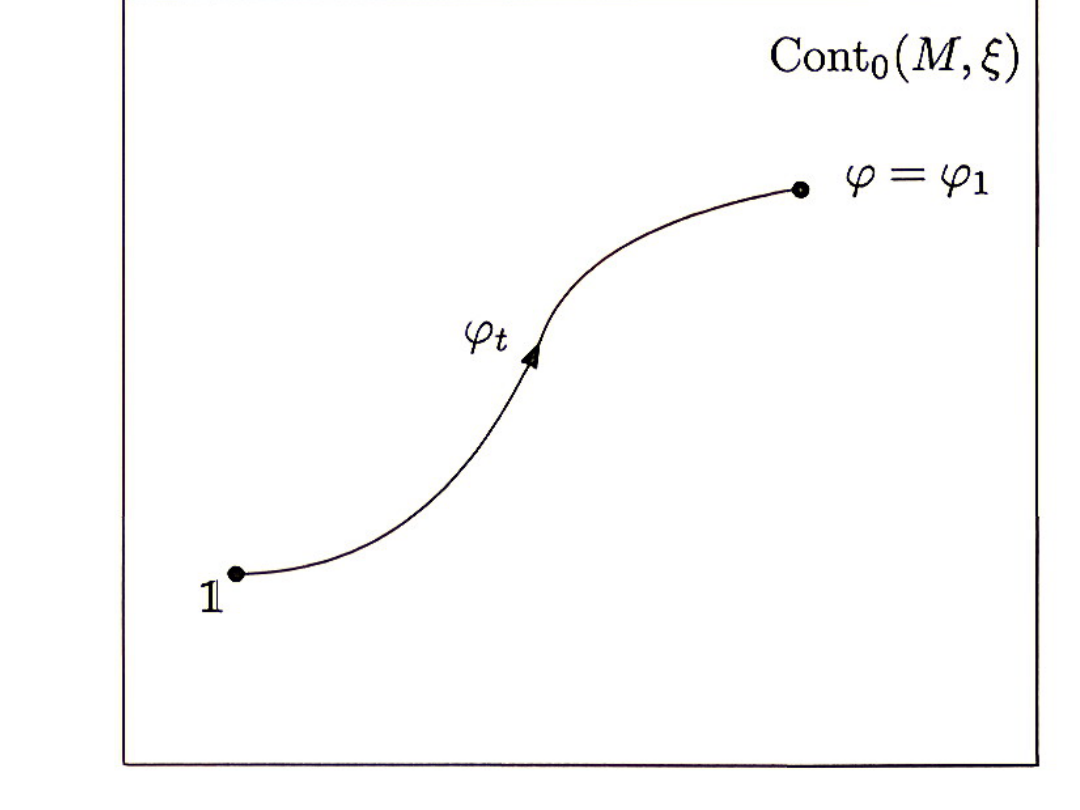
\includegraphics[width=0.50\linewidth]{figures/fig_p084_1.png}
  \caption*{图 3.14\quad $\Op{Cont}_0(M,\xi)$ 中的一条同痕（道路）
  （原书 p.76, Figure 3.14）}
\end{figure}

下面这个结果相当深刻，光滑情形下归功于 T. Rybicki [190]；对于更低的
正则性，相同结论出现在 [219] 以及 Y.-G. Oh 近期的工作 [172] 中。

\begin{wthm}{3.5.1}
对任意闭切触流形 $(M,\xi)$，切触同胚群 $\Op{Cont}(M,\xi)$ 是单群。
\end{wthm}

% [Tutor Note: 原文疑误（存疑）——对被证明为单群的通常是切触同胚群的恒等
% 分支 $\Op{Cont}_0(M,\xi)$（Banyaga–Rybicki 型定理）；若定理 3.5.1 字面上
% 指整个 $\Op{Cont}(M,\xi)$，则当 $\Op{Cont}$ 不连通时，其真子群
% $\Op{Cont}_0$ 将在单群中成为非平凡正规子群，产生矛盾。原文紧接着的一段也正是
% 拿 $\Op{Cont}_0(M,\xi)$ 与 $\Op{Ham}$ 作比较。建议按 $\Op{Cont}_0$ 理解。
% 已记入 review_ch03.md（标注「存疑」）。]

% >>> p085
与定理 1.7.1 相比较，上述单性表明 $\Op{Cont}_0(M,\xi)$ 更像辛几何中的
哈密顿微分同胚群 $\Op{Ham}$，而不是辛同胚群单位分支 $\Op{Symp}_0$ 的身份
（回忆由定理 1.7.2，$\Op{Ham}$ 一般不等于 $\Op{Symp}_0$）。下述命题揭示了
$\Op{Cont}_0(M,\xi)$ 的哈密顿特征。

\begin{wprop}{3.5.1}
给定切触流形 $(M,\xi=\ker\alpha)$ 以及
$\Op{Cont}_0(M,\xi)$ 中的同痕
$\varphi=\{\varphi_t\}_{t\in[0,1]}$，存在唯一的函数
$h:[0,1]\times M\to\R$ 在下述意义下「生成」$\varphi$：同痕 $\varphi$ 是由
向量场 $X_t$ 积分得到的，而 $X_t$ 满足如下方程
\begin{equation}\tag{3.30}
  h_t=\alpha(X_t),\qquad
  \dd h_t=\dd h_t(R_\alpha)\alpha-\iota_{X_t}\dd\alpha,
\end{equation}
其中 $R_\alpha$ 表示关于切触 $1$-形式 $\alpha$ 的 Reeb 向量场。
\end{wprop}

命题 3.5.1 给出的函数 $h$ 称为 $\varphi$ 的\textbf{切触哈密顿函数}
（contact Hamiltonian function，关于切触 $1$-形式 $\alpha$）。

\begin{wrem}{3.5.3}
使得 $\Op{Cont}_0(M,\xi)$ 中同痕 $\{\varphi_t\}_{t\in[0,1]}$ 得以积分的
向量场 $X_t$，由下述方程解出：
\begin{equation}\tag{3.31}
  \frac{\dd\varphi_t}{\dd t}=X_t\circ\varphi_t,
\end{equation}
且这与切触 $1$-形式的选择无关。只有转到函数层面时，才需要选取切触
$1$-形式。这个向量场 $X_t$ 称为\textbf{切触向量场}
（contact vector field）。
\end{wrem}

% [Tutor Note: 易错预警——(3.30) 的符号约定务必与 Cartan 公式对照：由
% $\mathcal{L}_{X_t}\alpha=\iota_{X_t}\dd\alpha+\dd\iota_{X_t}\alpha
% =\eta_t\alpha$ 及 (3.34) 的 $\eta_t=\dd h_t(R_\alpha)$，立刻得到
% $\dd h_t=\dd h_t(R_\alpha)\alpha-\iota_{X_t}\dd\alpha$。不少文献把接触
% 哈密顿向量场定义为满足
% $\dd h=\dd h(R_\alpha)\alpha+\iota_{X}\dd\alpha$，两者相差 $X$ 的符号；
% 引用公式时先把 $\alpha$ 的符号与 $R_\alpha$ 的归一化对齐。]

\begin{wexam}{3.5.3}
给定切触流形 $(M,\xi=\ker\alpha)$，若把 Reeb 流
$\{\varphi^t_{R_\alpha}\}_{t\in[0,1]}$ 看作 $\Op{Cont}_0(M,\xi)$ 中的
一条道路，则相应的切触哈密顿函数为 $h_t\equiv1$。方程 (3.30) 由定义方程
(3.2) 立得。当然，若考虑 $h_t\equiv s$（$s\in\R$ 为任意常数），则
$\Op{Cont}_0(M,\xi)$ 中相应的同痕是重新尺度化后的 Reeb 流
$\{\varphi^{st}_{R_\alpha}\}_{t\in[0,1]}$。注意这与（辛的）哈密顿动力学
非常不同：在辛流形上，任何常值函数都生成恒等映射。\hfill$//$
\end{wexam}

\begin{wproof}[命题 3.5.1 的证明]
从 (3.31) 的切触向量场 $X_t$ 出发。考虑 Lie 导数
$\mathcal{L}_{X_t}\alpha$，有
\begin{equation}\tag{3.32}
  \mathcal{L}_{X_t}\alpha
  =\left.\frac{\dd}{\dd s}\right|_{s=t}\varphi_s^*\alpha=\eta_t\alpha,
\end{equation}
其中 $\eta_t:M\to\R$ 是某个（待定的）函数。由 Cartan 公式，(3.32) 等价于
\begin{equation}\tag{3.33}
  \iota_{X_t}\dd\alpha+\dd\iota_{X_t}\alpha=\eta_t\alpha .
\end{equation}
% >>> p086
把 $R_\alpha$ 代入 (3.33)，得到
\begin{equation}\tag{3.34}
  (\iota_{X_t}\dd\alpha+\dd\iota_{X_t}\alpha)(R_\alpha)
  =0+\dd\bigl(\alpha(X_t)\bigr)(R_\alpha)=\eta_t .
\end{equation}
令 $h_t=\alpha(X_t)$（于是 (3.30) 的第一个方程得到满足），便由 (3.33)
得到 (3.30) 的第二个方程。
\end{wproof}

% [Tutor Note: 含糊点拨——命题 3.5.1 的「唯一性」部分证明中未加说明：给定
% 同痕，$X_t$ 由 (3.31) 唯一确定，从而 $h_t=\alpha(X_t)$ 唯一；反之给定
% $h_t$，(3.30) 的第二式给出 $\iota_{X_t}\dd\alpha
% =\dd h_t(R_\alpha)\alpha-\dd h_t$，由 $\dd\alpha|_\xi$ 非退化可唯一解出
% $X_t$ 的 $\xi$-分量，再由 $h_t=\alpha(X_t)$ 定出 Reeb 分量。证明只验证了
% 存在性，唯一性需补这一小步。]

命题 3.5.1 的重要性在于，人们可以系统地构造切触流形 $(M,\xi)$ 上的切触
同胚：从任意函数 $h:[0,1]\times M\to\R$ 出发，由 (3.30) 解出 $X_t$
（注意 (3.30) 的两个方程唯一确定 $X_t$），再把 $X_t$ 积分成同痕
$\{\varphi_t\}_{t\in[0,1]}$。所求的切触同胚就是该同痕的时间 $1$ 映射。若要
得到严格切触同胚，回到命题 3.5.1 的证明，可以先得到一列严格切触同胚构成的
同痕：由 (3.33) 与 (3.34)，只需取函数 $h:[0,1]\times M\to\R$ 使得
$\eta_t=\dd h_t(R_\alpha)=0$，即 $h_t$ 沿 Reeb 向量场不变。总之，这回答了
问题 3.1.1 中的 (ii)。

下述练习从同痕复合的角度，展示了切触哈密顿动力学与辛哈密顿动力学之间的另
一相似之处。

\begin{wexer}{3.5.1}（[165] 中引理 2.2）
给定切触流形 $(M,\xi=\ker\alpha)$，设 $h_t$ 是生成
$\Op{Cont}_0(M,\xi)$ 中同痕 $\psi=\{\psi_t\}$ 的切触哈密顿函数，且对某
共形因子 $\kappa(\psi_t)$ 有
$\psi^*\alpha=\ee^{\kappa(\psi_t)}\alpha$；又设 $g_t$ 是生成
$\Op{Cont}_0(M,\xi)$ 中同痕 $\varphi=\{\varphi_t\}$ 的切触哈密顿函数。
则 $h_t+(\ee^{\kappa(\psi_t)}g_t)\circ(\psi_t^{-1})$ 生成复合
$\psi\circ\varphi=\{\psi_t\circ\varphi_t\}$（参看方程 (1.17)）。此外，
复合 $\psi^{-1}\circ\varphi$ 由
$\ee^{-\kappa(\psi_t)}\bigl((g_t-h_t)\circ\psi_t\bigr)$ 生成。
\end{wexer}

% [Tutor Note: 含糊点拨——习题 3.5.1 是 §3.7「可序性」的代数基础：由第一
% 条结论，若把生成函数 $h_t$ 平移一个常数 $s$，则同痕被 Reeb 流
% $\varphi^{st}_{R_\alpha}$ 扭曲（见 §3.7 的 (3.42)）；由第二条结论，两个
% 同痕之差（之差）的生成函数可用来比较同痕的大小。核对时注意复合次序与
% $\psi_t^{-1}$、$\psi_t$ 的左右位置。]

切触哈密顿动力学与辛哈密顿动力学的最后一个相似之处，来自微分同胚与子流形
之间的转化：例如，辛流形 $(M,\omega)$ 上的辛同胚 $\varphi$ 与扭积
$(M\times M,\pi_1^*\omega-\pi_2^*\omega)$ 中的拉格朗日子流形
$\mathrm{graph}(\varphi)$ 之间的转化（见例 1.6.2）。

\begin{wexam}{3.5.4}
设 $(M,\xi=\ker\alpha)$ 是 $2n+1$ 维切触流形。考虑如下
$(4n+3)$ 维流形：$M\times M\times\R$，配以 $1$-形式
\begin{equation}\tag{3.35}
  \beta=-\ee^{\pi_\R}\pi_1^*\alpha+\pi_2^*\alpha,
\end{equation}
其中 $\pi_\R:M\times M\times\R\to\R$ 与 $\pi_i:M\times M\times\R\to M$
（$i=1,2$）是自然投影。

我们来确认 $\beta$ 是 $M\times M\times\R$ 上的切触 $1$-形式。在局部坐标
$(m_1,m_2,r)\in M\times M\times\R$ 中，为简单起见记 $\ee^{\pi_\R}=\ee^r$。
由 (3.35) 中 $\beta$ 的定义，有
\begin{align*}
  \beta\wedge(\dd\beta)^{2n+1}
  &=\bigl(-\ee^r\pi_1^*\alpha+\pi_2^*\alpha\bigr)
   \wedge\Bigl(-\ee^r\bigl(\dd r\wedge\pi_1^*\alpha+\pi_1^*\dd\alpha\bigr)
   +\pi_2^*\dd\alpha\Bigr)^{2n+1}\\
  &=C\cdot\ee^{(n+1)r}\dd r\wedge\pi_1^*\alpha
   \wedge(\pi_1^*\dd\alpha)^n\wedge\pi_2^*\alpha
   \wedge(\pi_2^*\dd\alpha)^n\\
  &=C\cdot\ee^{(n+1)r}\dd r\wedge\pi_1^*\bigl(\alpha\wedge(\dd\alpha)^n\bigr)
   \wedge\pi_2^*\bigl(\alpha\wedge(\dd\alpha)^n\bigr),
\end{align*}
% >>> p087
其中 $C$ 是正常数。因此 $\beta\wedge(\dd\beta)^{2n+1}$ 是
$M\times M\times\R$ 上的体积形式，这说明 $\beta$ 是切触 $1$-形式。

读者或许会好奇 $\beta$ 的 Reeb 向量场 $R_\beta$。考虑向量场
$X:=(0,R_\alpha,0)$，其中 $R_\alpha$ 是 $(M,\xi=\ker\alpha)$ 的 Reeb
向量场，则可验证方程 (3.2)：
\[
  \beta(X)=-\ee^r\pi_1^*\alpha(X)+\pi_2^*\alpha(X)
  =\alpha(R_\alpha)=1,
\]
以及
\[
  \dd\beta(X,\cdot)
  =\bigl(-\ee^r(\dd r\wedge\pi_1^*\alpha+\pi_1^*\dd\alpha)
   +\pi_2^*\dd\alpha\bigr)\bigl((0,R_\alpha,0),\cdot\bigr)
  =\dd\alpha(R_\alpha,\cdot)=0 .
\]
因此 $R_\beta=X=(0,R_\alpha,0)$。

对任意满足 $\varphi^*\alpha=\ee^{\kappa(\varphi)}\alpha$（某共形因子
$\ee^{\kappa(\varphi)}$）的 $M$ 上切触同胚 $\varphi$，考虑如下子流形：
\begin{equation}\tag{3.36}
  \overline{\mathrm{graph}}(\varphi)
  :=\bigl\{(x,\varphi(x),\kappa(\varphi)(x))\ \big|\ x\in M\bigr\}
  \subset M\times M\times\R .
\end{equation}
我们断言 $\overline{\mathrm{graph}}(\varphi)$ 是切触流形
$(M\times M\times\R,\xi=\ker\beta)$ 的勒让德子流形。事实上，维数条件自动
满足。记 $i:\overline{\mathrm{graph}}(\varphi)\to M\times M\times\R$ 为
嵌入映射。固定
$p=(x,\varphi(x),\kappa(\varphi)(x))\in\overline{\mathrm{graph}}(\varphi)$，
对任意切向量
$Y\in T_p(\overline{\mathrm{graph}}(\varphi))$，有
\begin{align*}
  i^*(\beta)(Y)
  &=i^*\bigl(-\ee^r\pi_1^*\alpha+\pi_2^*\alpha\bigr)(Y)\\
  &=-\ee^{\kappa(\varphi)(x)}\alpha\bigl((\pi_1\circ i)_*(Y)\bigr)
   +\alpha\bigl((\pi_2\circ i)_*(Y)\bigr)\\
  &=-\ee^{\kappa(\varphi)(x)}\alpha\bigl((\pi_1\circ i)_*(Y)\bigr)
   +\alpha\bigl(\varphi_*((\pi_1\circ i)_*(Y))\bigr)=0,
\end{align*}
其中最后一个等号来自共形因子的定义性质。因此我们断定
$\overline{\mathrm{graph}}(\varphi)$ 的切空间满足
$T(\overline{\mathrm{graph}}(\varphi))\subset\xi(=\ker\beta)$。\hfill$//$
\end{wexam}

% [Tutor Note: 术语提示——$\overline{\mathrm{graph}}(\varphi)$ 之所以加
% 上划线，是因为它把通常的「图」$(x,\varphi(x))$ 提升到
% $M\times M\times\R$ 中，用额外坐标 $\kappa(\varphi)(x)$ 记录共形因子。
% 这正是切触同胚的图成为勒让德子流形的关键：辛情形下用
% $(M\times M,\pi_1^*\omega-\pi_2^*\omega)$，切触情形下则需把
% $-\ee^r\pi_1^*\alpha$ 与 $\pi_2^*\alpha$ 相加，并以 $r=\kappa(\varphi)$
% 补偿共形因子。]
